\documentclass{article}
\usepackage[utf8]{inputenc}
\usepackage{hyperref}
\usepackage{graphicx}
\usepackage{listings}
\usepackage{amssymb}
\usepackage{color}
\usepackage{xcolor}
\usepackage{indentfirst}

\lstset{frame=single,backgroundcolor=\color{lightgray}}

\newcommand{\menu}[1]{\colorbox{yellow}{\texttt{#1}}}
\newcommand{\wizard}[1]{\colorbox{green}{\texttt{#1}}}
\newcommand{\inkscape}[2]{
\IfFileExists{jeter_svg_#1.png}{}{\immediate\write18{inkscape -z --export-png=jeter_svg_#1.png #1.svg}}
\begin{center}
\includegraphics[#2]{jeter_svg_#1.png}
\end{center}
}


\def\emf{\textbf{EMF} }
\date{\today}
\title{EMF Notebook}
\author{Pierre Lindenbaum\\\href{https://twitter.com/yokofakun}{@yokofakun}\\\url{http://plindenbaum.blogspot.com} }

\begin{document}
\maketitle

\begin{abstract}
\emf (The Eclipse Modeling Framework) is a Java framework and \textbf{code generation facility} for building tools and other applications based on a structured model.  Once you specify an EMF model, the \textbf{EMF generator} can create a corresponding set of Java implementation classes. In the following tutorial I'm going to generate a simple-and-stupid \href{https://en.wikipedia.org/wiki/Laboratory_information_management_system}{LIMS}.
\end{abstract}

We're going to create an interface for a simple-and-stupid \href{https://en.wikipedia.org/wiki/Laboratory_information_management_system}{LIMS}.
\inkscape{lims}{scale=0.5}

\begin{itemize}
\item A laboratory contains a list of \textbf{Families}
\item A laboratory contains a list of \textbf{Sequencers}
\item a family contains a list of \textbf{Individuals}
\item an Individual contains a list of  \textbf{Samples}
\item a Sequencer contains a list of  \textbf{Runs}
\item a Run contains a list of  \textbf{Sequenced} which links to a Sample.
\end{itemize}

At the end of this tutorial, we're going to generate the following heavy client for our model:\\
\begin{center}
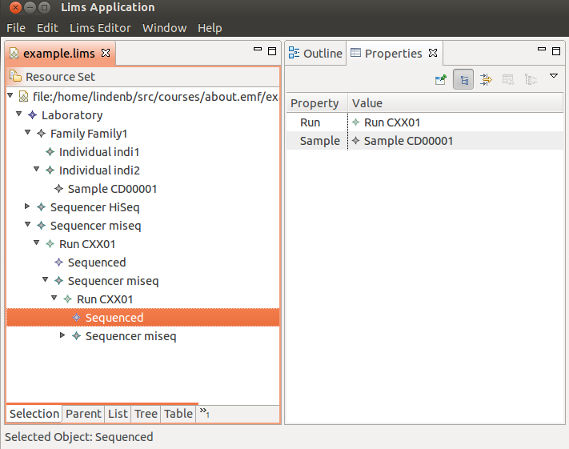
\includegraphics[scale=0.6]{example.png}
\end{center}

\section{Install the EMF plugins for Eclipse}

see \url{http://wiki.eclipse.org/EMF/Installation#Install_EMF}.

\section{Creating the Model}
A model is created and defined in the \textbf{Ecore} format, which is basically a sub-set of UML Class diagrams.\\
\subsection{Create the Project}
\begin{itemize}
\item Open Eclipse
\item Menu \menu{File $\rightarrow$  New  $\rightarrow$ New Project... $\rightarrow$ Empty EMF Project}
\item Name the project \textbf{EMF03-Model}
\end{itemize}
\subsection{Create the ECore model}
create a new 'ECore' file in the model folder in your new modeling project.
\begin{itemize}
\item Menu \menu{File $\rightarrow$  New  $\rightarrow$ Other.. $\rightarrow$ ECore Model}
\item Wizard: select the folder \textbf{EMF03-Model/model}.
\item Wizard: set the filename as \textbf{lims.ecore}.
\item Wizard: set Model Object as  \textbf{EPackage}.
\item Menu \menu{Window  $\rightarrow$ Show View $\rightarrow$ Other $\rightarrow$ Properties}
\end{itemize}

\input{jeter01.tex}
All in one, the file \textbf{lims.ecore} looks like this:
\lstinputlisting[language=xml,breaklines=true,numbers=left]{model/lims.ecore}

\section{GenModel}
We're going to generate the \textbf{Genmodel} for our model. The \textbf{Genmodel} contains additional information for the codegeneration, e.g. the path and file information. 
\subsection{Create the GenModel Project}
\begin{itemize}
\item Menu \menu{File $\rightarrow$  New  $\rightarrow$ New Project... $\rightarrow$ EMF Generator Project}
\item Select the folder \textbf{EMF03-Model/model}
\item Set the file name to \textbf{lims.genmodel}
\item select a \wizard{"Model Importer": "Ecore model"}
\item import the model "\texttt{URI: platform:/resource/EMF03/model/lims.ecore}"
\end{itemize}

\subsection{Edit the GenModel Project}
In the tree view of the \textbf{Genmodel}, click on the root node and edit its properties:
\begin{itemize}
\item set \menu{All $\rightarrow$  Runtime Platform  $\rightarrow$ } to  \textbf{"RCP"}.
\end{itemize}

 click on the package node 'Lims' and edit its properties:
\begin{itemize}
\item set \menu{All $\rightarrow$  BasePackage  $\rightarrow$ } to  "com.github.lindenb.lims".
\end{itemize}


\lstinputlisting[language=xml,breaklines=true,numbers=left]{model/lims.genmodel}

\section{Generating the code}
In the tree view of the \textbf{Genmodel}, right click the root node: \menu{Generate All}: four new Eclipse plugins have been created:
\begin{itemize}
\item{Model}: contains the classes to create the instances of our model.
\item{EMF03.edit} : classes to display a model in a UI (labels... )
\item{EMF03.editor}: The editor plugin is a generated example editor to create and modify instances of a model.
\item{EMF03.tests}: The test plugin contains templates to write tests for a model.
\end{itemize}

Here is an example of the interface \textbf{\texttt{com.github.lindenb.lims.Lims.Family}} generated by EMF:
\begin{lstlisting}[language=java,basicstyle=\tiny,breaklines=true,numbers=left]
package com.github.lindenb.lims.Lims;

import org.eclipse.emf.common.util.EList;

import org.eclipse.emf.ecore.EObject;

/**
 * A representation of the model object '<em><b>Family</b></em>'.
 *
 * The following features are supported:
 * <ul>
 *   <li>{@link com.github.lindenb.lims.Lims.Family#getName <em>Name</em>}</li>
 *   <li>{@link com.github.lindenb.lims.Lims.Family#getIndividuals <em>Individuals</em>}</li>
 *   <li>{@link com.github.lindenb.lims.Lims.Family#getLaboratory <em>Laboratory</em>}</li>
 * </ul>
 *
 * @see com.github.lindenb.lims.Lims.LimsPackage#getFamily()
 * @model
 * @generated
 */
public interface Family extends EObject
{
	/**
	 * Returns the value of the '<em><b>Name</b></em>' attribute.
	 * If the meaning of the '<em>Name</em>' attribute isn't clear,
	 * there really should be more of a description here...
	 * @return the value of the '<em>Name</em>' attribute.
	 * @see #setName(String)
	 * @see com.github.lindenb.lims.Lims.LimsPackage#getFamily_Name()
	 * @model required="true"
	 * @generated
	 */
	String getName();

	/**
	 * Sets the value of the '{@link com.github.lindenb.lims.Lims.Family#getName <em>Name</em>}' attribute.
	 * @param value the new value of the '<em>Name</em>' attribute.
	 * @see #getName()
	 * @generated
	 */
	void setName(String value);

	/**
	 * Returns the value of the '<em><b>Individuals</b></em>' containment reference list.
	 * The list contents are of type {@link com.github.lindenb.lims.Lims.Individual}.
	 * It is bidirectional and its opposite is '{@link com.github.lindenb.lims.Lims.Individual#getFamily <em>Family</em>}'.
	 * If the meaning of the '<em>Individuals</em>' containment reference list isn't clear,
	 * there really should be more of a description here...
	 * @return the value of the '<em>Individuals</em>' containment reference list.
	 * @see com.github.lindenb.lims.Lims.LimsPackage#getFamily_Individuals()
	 * @see com.github.lindenb.lims.Lims.Individual#getFamily
	 * @model opposite="family" containment="true"
	 * @generated
	 */
	EList<Individual> getIndividuals();

	/**
	 * Returns the value of the '<em><b>Laboratory</b></em>' container reference.
	 * It is bidirectional and its opposite is '{@link com.github.lindenb.lims.Lims.Laboratory#getFamilies <em>Families</em>}'.
	 * If the meaning of the '<em>Laboratory</em>' container reference isn't clear,
	 * there really should be more of a description here...
	 * @return the value of the '<em>Laboratory</em>' container reference.
	 * @see #setLaboratory(Laboratory)
	 * @see com.github.lindenb.lims.Lims.LimsPackage#getFamily_Laboratory()
	 * @see com.github.lindenb.lims.Lims.Laboratory#getFamilies
	 * @model opposite="families" required="true" transient="false"
	 * @generated
	 */
	Laboratory getLaboratory();

	/**
	 * Sets the value of the '{@link com.github.lindenb.lims.Lims.Family#getLaboratory <em>Laboratory</em>}' container reference.
	 * @param value the new value of the '<em>Laboratory</em>' container reference.
	 * @see #getLaboratory()
	 * @generated
	 */
	void setLaboratory(Laboratory value);

} // Family
\end{lstlisting}
and the implementation of the interface: \textbf{\texttt{com.github.lindenb.lims.Lims.impl.FamilyImpl}} :
\begin{lstlisting}[language=java,basicstyle=\tiny,breaklines=true,numbers=left]
package com.github.lindenb.lims.Lims.impl;

import com.github.lindenb.lims.Lims.Family;
import com.github.lindenb.lims.Lims.Individual;
import com.github.lindenb.lims.Lims.Laboratory;
import com.github.lindenb.lims.Lims.LimsPackage;

import java.util.Collection;

import org.eclipse.emf.common.notify.Notification;
import org.eclipse.emf.common.notify.NotificationChain;

import org.eclipse.emf.common.util.EList;

import org.eclipse.emf.ecore.EClass;
import org.eclipse.emf.ecore.InternalEObject;

import org.eclipse.emf.ecore.impl.ENotificationImpl;
import org.eclipse.emf.ecore.impl.EObjectImpl;

import org.eclipse.emf.ecore.util.EObjectContainmentWithInverseEList;
import org.eclipse.emf.ecore.util.EcoreUtil;
import org.eclipse.emf.ecore.util.InternalEList;

/**
 * An implementation of the model object '<em><b>Family</b></em>'.
 * The following features are implemented:
 * <ul>
 *   <li>{@link com.github.lindenb.lims.Lims.impl.FamilyImpl#getName <em>Name</em>}</li>
 *   <li>{@link com.github.lindenb.lims.Lims.impl.FamilyImpl#getIndividuals <em>Individuals</em>}</li>
 *   <li>{@link com.github.lindenb.lims.Lims.impl.FamilyImpl#getLaboratory <em>Laboratory</em>}</li>
 * </ul>
 *
 * @generated
 */
public class FamilyImpl extends EObjectImpl implements Family
{
	/**
	 * The default value of the '{@link #getName() <em>Name</em>}' attribute.
	 * @see #getName()
	 * @generated
	 * @ordered
	 */
	protected static final String NAME_EDEFAULT = null;

	/**
	 * The cached value of the '{@link #getName() <em>Name</em>}' attribute.
	 * @see #getName()
	 * @generated
	 * @ordered
	 */
	protected String name = NAME_EDEFAULT;

	/**
	 * The cached value of the '{@link #getIndividuals() <em>Individuals</em>}' containment reference list.
	 * @see #getIndividuals()
	 * @generated
	 * @ordered
	 */
	protected EList<Individual> individuals;

	/**
	 * @generated
	 */
	protected FamilyImpl()
	{
		super();
	}

	/**
	 * @generated
	 */
	@Override
	protected EClass eStaticClass()
	{
		return LimsPackage.Literals.FAMILY;
	}

	/**
	 * @generated
	 */
	public String getName()
	{
		return name;
	}

	/**
	 * @generated
	 */
	public void setName(String newName)
	{
		String oldName = name;
		name = newName;
		if (eNotificationRequired())
			eNotify(new ENotificationImpl(this, Notification.SET, LimsPackage.FAMILY__NAME, oldName, name));
	}

	/**
	 * @generated
	 */
	public EList<Individual> getIndividuals()
	{
		if (individuals == null)
		{
			individuals = new EObjectContainmentWithInverseEList<Individual>(Individual.class, this, LimsPackage.FAMILY__INDIVIDUALS, LimsPackage.INDIVIDUAL__FAMILY);
		}
		return individuals;
	}

	/**
	 * @generated
	 */
	public Laboratory getLaboratory()
	{
		if (eContainerFeatureID() != LimsPackage.FAMILY__LABORATORY) return null;
		return (Laboratory)eContainer();
	}

	/**
	 * @generated
	 */
	public NotificationChain basicSetLaboratory(Laboratory newLaboratory, NotificationChain msgs)
	{
		msgs = eBasicSetContainer((InternalEObject)newLaboratory, LimsPackage.FAMILY__LABORATORY, msgs);
		return msgs;
	}

	/**
	 * @generated
	 */
	public void setLaboratory(Laboratory newLaboratory)
	{
		if (newLaboratory != eInternalContainer() || (eContainerFeatureID() != LimsPackage.FAMILY__LABORATORY && newLaboratory != null))
		{
			if (EcoreUtil.isAncestor(this, newLaboratory))
				throw new IllegalArgumentException("Recursive containment not allowed for " + toString());
			NotificationChain msgs = null;
			if (eInternalContainer() != null)
				msgs = eBasicRemoveFromContainer(msgs);
			if (newLaboratory != null)
				msgs = ((InternalEObject)newLaboratory).eInverseAdd(this, LimsPackage.LABORATORY__FAMILIES, Laboratory.class, msgs);
			msgs = basicSetLaboratory(newLaboratory, msgs);
			if (msgs != null) msgs.dispatch();
		}
		else if (eNotificationRequired())
			eNotify(new ENotificationImpl(this, Notification.SET, LimsPackage.FAMILY__LABORATORY, newLaboratory, newLaboratory));
	}

	/**
	 * @generated
	 */
	@SuppressWarnings("unchecked")
	@Override
	public NotificationChain eInverseAdd(InternalEObject otherEnd, int featureID, NotificationChain msgs)
	{
		switch (featureID)
		{
			case LimsPackage.FAMILY__INDIVIDUALS:
				return ((InternalEList<InternalEObject>)(InternalEList<?>)getIndividuals()).basicAdd(otherEnd, msgs);
			case LimsPackage.FAMILY__LABORATORY:
				if (eInternalContainer() != null)
					msgs = eBasicRemoveFromContainer(msgs);
				return basicSetLaboratory((Laboratory)otherEnd, msgs);
		}
		return super.eInverseAdd(otherEnd, featureID, msgs);
	}

	/**
	 * @generated
	 */
	@Override
	public NotificationChain eInverseRemove(InternalEObject otherEnd, int featureID, NotificationChain msgs)
	{
		switch (featureID)
		{
			case LimsPackage.FAMILY__INDIVIDUALS:
				return ((InternalEList<?>)getIndividuals()).basicRemove(otherEnd, msgs);
			case LimsPackage.FAMILY__LABORATORY:
				return basicSetLaboratory(null, msgs);
		}
		return super.eInverseRemove(otherEnd, featureID, msgs);
	}

	/**
	 * @generated
	 */
	@Override
	public NotificationChain eBasicRemoveFromContainerFeature(NotificationChain msgs)
	{
		switch (eContainerFeatureID())
		{
			case LimsPackage.FAMILY__LABORATORY:
				return eInternalContainer().eInverseRemove(this, LimsPackage.LABORATORY__FAMILIES, Laboratory.class, msgs);
		}
		return super.eBasicRemoveFromContainerFeature(msgs);
	}

	/**
	 * @generated
	 */
	@Override
	public Object eGet(int featureID, boolean resolve, boolean coreType)
	{
		switch (featureID)
		{
			case LimsPackage.FAMILY__NAME:
				return getName();
			case LimsPackage.FAMILY__INDIVIDUALS:
				return getIndividuals();
			case LimsPackage.FAMILY__LABORATORY:
				return getLaboratory();
		}
		return super.eGet(featureID, resolve, coreType);
	}

	/**
	 * @generated
	 */
	@SuppressWarnings("unchecked")
	@Override
	public void eSet(int featureID, Object newValue)
	{
		switch (featureID)
		{
			case LimsPackage.FAMILY__NAME:
				setName((String)newValue);
				return;
			case LimsPackage.FAMILY__INDIVIDUALS:
				getIndividuals().clear();
				getIndividuals().addAll((Collection<? extends Individual>)newValue);
				return;
			case LimsPackage.FAMILY__LABORATORY:
				setLaboratory((Laboratory)newValue);
				return;
		}
		super.eSet(featureID, newValue);
	}

	/**
	 * @generated
	 */
	@Override
	public void eUnset(int featureID)
	{
		switch (featureID)
		{
			case LimsPackage.FAMILY__NAME:
				setName(NAME_EDEFAULT);
				return;
			case LimsPackage.FAMILY__INDIVIDUALS:
				getIndividuals().clear();
				return;
			case LimsPackage.FAMILY__LABORATORY:
				setLaboratory((Laboratory)null);
				return;
		}
		super.eUnset(featureID);
	}

	/**
	 * @generated
	 */
	@Override
	public boolean eIsSet(int featureID)
	{
		switch (featureID)
		{
			case LimsPackage.FAMILY__NAME:
				return NAME_EDEFAULT == null ? name != null : !NAME_EDEFAULT.equals(name);
			case LimsPackage.FAMILY__INDIVIDUALS:
				return individuals != null && !individuals.isEmpty();
			case LimsPackage.FAMILY__LABORATORY:
				return getLaboratory() != null;
		}
		return super.eIsSet(featureID);
	}

	/**
	 * @generated
	 */
	@Override
	public String toString()
	{
		if (eIsProxy()) return super.toString();

		StringBuffer result = new StringBuffer(super.toString());
		result.append(" (name: ");
		result.append(name);
		result.append(')');
		return result.toString();
	}

} //FamilyImpl
\end{lstlisting}

\section{Create a new eclipse product}
\begin{itemize}
\item Menu \menu{File $\rightarrow$  New  $\rightarrow$ Other... $\rightarrow$ Product Configuration}
\item Wizard: set parent folder: \textbf{EMF03/model}
\item Wizard: set the file name: "lims.product".
\item Wizard: Ask to create a basic config
\end{itemize}
Open the editor for 'lims.product".
\begin{itemize}
\item in  \wizard{Overview/Product Definition/Product} $\rightarrow$ \wizard{create a new product}.  \wizard{Defining plugin}:"EMF03",  \wizard{product ID}: "lims",  \wizard{Application}: \texttt{"EMF03.editor.LimsEditorEditorAdvisorApplication"}.
\item in Depedencies/Plugins and fragments: add EMF03, EMF03.edit, EMF03.editor
\item check \wizard{"include optional dependencies"}
\item click  \wizard{"Add required plug-in"}
\item in  \wizard{Lauching/Program Launcher} set  \wizard{Launcher Name} to "lims".
\end{itemize}

The content of the product file is displayed below:
\lstinputlisting[language=xml,breaklines=true,numbers=left]{model/lims.product}

\section{Generating the Eclipse Product}
\begin{itemize}
\item \menu{File  $\rightarrow$ Export  $\rightarrow$ Eclipse Product}.
\item Set \wizard{configuration}: "EMF03/model/lims.product" .
\item Set the \wizard{destination directory}.
\item Uncheck \wizard{"Generate metadata repository"}.
\item \wizard{"Finish"} 
\end{itemize}
Congratulations, your client has been generated.
\section{Running the Lims editor}
Go to the generated application directory and run:
\begin{lstlisting}[language=bash]
$ cd /path/to/GENERATED
$ ./lims &
\end{lstlisting}

Here is a screenshot of the generated 'lims' application:

\begin{center}
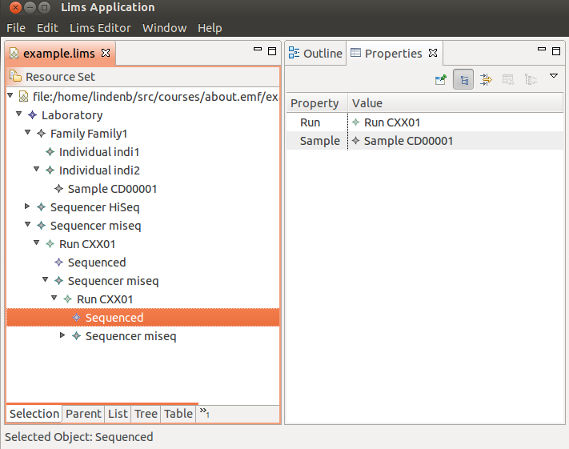
\includegraphics[scale=0.6]{example.png}
\end{center}

Here is an example of a data file handled by the 'lims' application:
\lstinputlisting[language=xml,breaklines=true,numbers=left]{example.lims}

That's it,

Pierre

\section{References}
\begin{itemize}
\item Source for this tutorial: \url{https://github.com/lindenb/courses/tree/master/about.emf}
\item The Eclipse Modeling Framework Overview : \url{http://help.eclipse.org/juno/index.jsp?topic=%2Forg.eclipse.emf.doc%2Freferences%2Foverview%2FEMF.html}
\item Eclipse Modeling Framework (EMF) - Tutorial : \url{http://www.vogella.com/articles/EclipseEMF/article.html}
\end{itemize}

\end{document}
